\chapter{Background and Previous Work}\label{previous_work}
Previous work and the background information needed for this
thesis is described in this chapter. We look at how microblogging activity
can be related to finance and stock market prediction \cite{bollen2011}, and how
sentiment can be used to predict stock markets.

This chapter contains related research, context knowledge and introduction to
the subjects discussed in this thesis. Twitter as a microblogging platform is
introduced in section \ref{previous_work:twitter}. Section
\ref{previous_work:sentiment}, describes sentiment analysis and what it can be used for.
Finance and trading is described in section
\ref{previous_work:finance}. In the last section, \ref{previous_work:trends}, of
this chapter trends are introduces. 

\section{Twitter}\label{previous_work:twitter}
Twitter is a social informations network. 
It's a real-time service for sharing and gathering small messages. These
messages can represent everything from a persons opinion of ice cream, to the
latest changes in the financial market or pictures from a Mars rover. 

At the core of Twitter\footnote{About Twitter: \url{https://twitter.com/about}}
you have the Tweet. The Tweet is a 140 character message. 
Tweets lets you communicate with other users, share photos and post all kinds of
information. The small size of the tweets are not a hindrance for the flow of
information. 

The fast growing messaging service handles 1.6 billion search queries every day.
In 2012 the 500 million users would generate 3.2 queries each, every day. 340 million tweets were posted every day. 
\footnote{Wikipedia: \url{http://en.wikipedia.org/wiki/Twitter}} 

Most medium and large companies have a presence on Twitter today. Posts can contain
any type of information, from promotional content to service status to
financial reports. \cite[p8]{annikajubbega11:twitter_driver_stock_price} says
that 77 of the Fortune 100 companies have a Twitter account. 

Companies use Twitter to communicate with customers. Customers can post
questions and feedback, while companies posts answers and information.
Questions can be asked with a specific hashtag(\#). Or with an at(@) sign to target a
specific user. This makes it easy to filter the messages, and therefore easier
to get in contact with the customer. The company Best Buy demonstrated the successfulness of
twitter in customer relations by answering questions with a specific hashtag. In
2009 they had answered nearly 20 thousand questions using twitter.
\cite[p1]{Li2013206} Market Intelligence is also a major aspect of the
microblogging sphere.

Twitter represents one of the largest and most dynamic datasets of user
generated content. Along with Facebook Twitter data is in real time. This has major
implications for anyone who are interested in sentiment, public opinion or
customer interaction. \cite[]{sperious11}

A typical tweet contains about 11 words and provides an opinion or state of
mind or a piece of information. Tweets can contain hashtags: '\#something',
Twitter handles:
'@username', or other adaptations of prefixes such as '\$STO' which represents a
stock. Different prefixes or tags (\$, \#, @) can easily distinguish
content of a tweet. This also makes it easier to search and classify the
content of tweets. Figure:\ref{fig:sto} and figure:\ref{fig:tweet1} are
examples of tweets as shown on Twitter.

The retrieval of tweets seems like a challenge. But Twitter has made this easy
by providing an API\footnote{API: Application programming interface}. With the
API you can write tweets and update the status of a user. But the best part of
the API is that it provides search capabilities. To get a certain subset of all
tweets, we can use the search function and view only the tweets we want. 

On the front page of Twitter we have the search function at the top right of
the page. The search provides the ability to specify which types of tweets you
want. And gives you the opportunity to find the information you are looking for. 

\begin{figure}[htb]
    \centering
    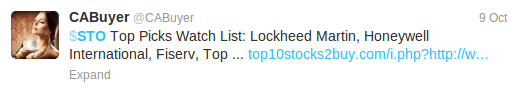
\includegraphics[width=\textwidth]{STO} 
    \caption{Typical tweet from Twitter.}
    \label{fig:sto}
\end{figure}

%\begin{figure}[htb]
%    \centering
%    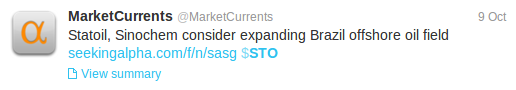
\includegraphics[width=\textwidth]{STO2} 
%    \caption{The text that shows under the image, image text.}
%    \label{fig:sto2}
%\end{figure}

\begin{figure}[htb]
    \centering
    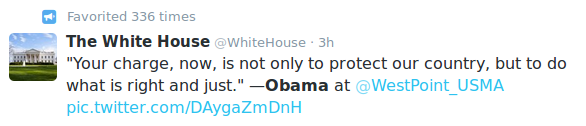
\includegraphics[width=\textwidth]{tweet1} 
    \caption{Typical tweet from Twitter.}
    \label{fig:tweet1}
\end{figure}

%\begin{figure}[htb]
%    \centering
%    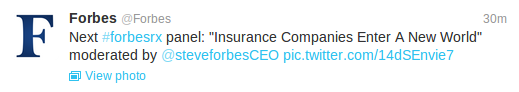
\includegraphics[width=\textwidth]{tweet2} 
%    \caption{The text that shows under the image, image text.}
%    \label{fig:tweet2}
%\end{figure}
%
%\begin{figure}[htb]
%    \centering
%    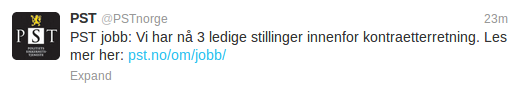
\includegraphics[width=\textwidth]{tweet3} 
%    \caption{The text that shows under the image, image text.}
%    \label{fig:tweet3}
%\end{figure}

\section{Sentiment}\label{previous_work:sentiment}

Opinion mining on the web is not new. In recent years it has
become attractive to traders. 
The use of Twitter and social media is increasing. Both in
business and with private users.
This means a surplus of raw data with
easy access. Companies all over the world has started to use social
networks to their benefit. The use of information from social media has become
part of the trend, although there are some drawbacks and shortcomings. Noise and
garbage is one of them. Even if you're right 80\% of the time, the last 20\% can
prove devastating. \cite[]{stevenson12:social_media_stock_pickers}

Sentiment broadly refers to a persons state of mind. Based on the opinion the
person will do optimistic or pessimistic choices. A positive mindset leads to
optimistic judgements of future events, and a negative state of mind leads to
pessimistic choices.
\cite[p4]{doukas10:sentiment_and_momentum}

The users may have different roles and intentions in different
communities in the microblogging sphere, \cite[]{java07}. 
A users intentions and its reasons for participation might be a factor in the sentiment analysis.

\subsection{What is Sentiment Analysis}
There are two main categories of approaches to sentiment detection. The first is
to use a classifier. The classifier can use methods such as Naive Bayes, maximum
entropy or support vector machine \cite[]{Li2013206}. These classifiers are
typical examples where it would be natural to use machine learning on
evolutionary algorithms to increase the classification correctness over time.
The second is the use of linguistic resources, such as corpora of negative and
positive words. The developed linguistic resources are used to classify the
sentiment of text, \cite[]{Li2013206}.

Li and Li has created a framework for sentiment analysis. The system
consists of four main steps  and is tested with experiments on twitter. 
	First they do topic detection, identifying and extracting the topics
mentioned in the tweet. 
	Secondly opinions are classified. The polarity, how positive a tweets is, of the opinion is decided and
the users impression is captured. 	
	Third, credibility is assessed. This creates a better summarization of the
expresser's credibility. 
	Fourth, step one, two, and three are aggregated to reflect the true opinion
and point of view.
	Combining the first three steps, in the fourth, results in a truer
reflection of the expresser's opinion. \cite[]{Li2013206} 

One way of classifying tweets is to use predefined lexicons of positive and
negative words. Consumer confidence and fluctuations of voting polls can be
tracked this way \cite[]{connor2010}.

The work of \cite[]{diakopoulos2010} describes a methodology for better
understanding of temporal dynamics of sentiment. 
The system uses visual representation to achieve this. 
This is investigated in the reaction to debate video.
	Further \cite[]{diakopoulos2010} detects sentiment pulse and controversial
topics with the help of visualisation and metrics. 
	\cite[]{diakopoulos2010} used crowdsourcing\footnote{Crowdsourcing is the
practice of obtaining needed services, ideas, or content by soliciting
contributions from a large group of people, and especially from an online
community, rather than from traditional employees or suppliers.
\url{http://en.wikipedia.org/wiki/Crowdsourcing}} to classify batches of tweets.
This was accomplished with Amazon Mechanical Turk, a crowdsourcing
site\footnote{Amazon Mechanical Turk (AMT): \url{https://www.mturk.com/mturk/}}.

\cite[]{barbosa10} explores the problem of noise in biased and noisy data. 
They focus on noisy labels and add features to the tweets to increase the
classification properties of the tweets. Objective tweets have very little
sentiment or no sentiment at all. To improve classification, tweets are
classified as objective of subjective. Then the subjective tweets, that have a
sentiment are classified as positive of negative. 

Classification of tweets can be generalised by using features. Features are
small elements of a tweet, such as monograms\footnote{Monogram, same as
Unigram}, bigrams, or part-of-speech tags. Bigrams are words consisting of two
words, monograms are words consisting of one word. An abstract representation of
a tweet would be beneficial to the classification. In this abstract
representation \cite[]{barbosa10} propose to use characteristics about how
tweets are written and meta-information about the words in tweets, meta-features and tweet syntax features that can further improve classification.
Meta-features are information about the tweet, such as location, language, and
number of retweets. Retweets are tweets that are posted again by other users.
The tweet syntax features are things such as hashtags, retweet, reply, links,
punctuation and emoticons \cite[]{barbosa10}. 

Challenges with sentiment and Twitter is described in another approach by 
\cite[]{becker13}. They explore techniques for contextual polarity
disambiguation and message polarity classification. Constrained and supervised
learning is used to create models for classification. They describe a system
that solves these tasks with the help of polarity lexicons and dependency
parsers. Expanded vocabulary is one of the main aspects of their success, as
they say in their findings: "We hypothesize this performance is largely due to
the expanded vocabulary obtained via unlabeled data and the richer syntactic
context captured with dependency path representations." \cite[]{becker13}

In contrast to \cite[]{becker13}, \cite[]{sperious11} has used distant
supervision and labeled propagation on a graph based data structure. The data
structure represents users with tweets as nodes. And tweets with bigrams,
monograms, hashtags, etc as subnodes of the tweets. A label propagation approach
rivals a model supervised with in-domain annotated tweets, and outperforms the
noisily supervised classifier, and a lexicon-based polarity ratio classifier.
\cite[]{sperious11} 

\subsection{Sentiment Analysis in Finance}
\cite[p2]{Brown20041} writes the following on over-reaction of investors: 
"\textit{He(Siegel (1992)) concludes that shifts in investor sentiment are correlated
with market returns around the crash. Intuitively, sentiment represents the
expectations of market participants relative to a norm: a bullish (bearish)
investor expects returns to be above (below) average, whatever ‘‘average’’ may
be."}. 
In the light of recent changes in the financial world, and the use
of sentiment from social media, the notion that opinions and sentiment of
investors and market actors affect the market is not a new observation.

Use of sentiment can potentially predict changes and trends in the market.
Bad news in an optimistic period creates cognitive dissonance in the small
investors. This impacts the market by slowing down the selling rate of loosing
stocks, \cite[p29]{doukas10:sentiment_and_momentum}.
Further we can see that optimistic sentiment has a 2\% monthly average return.
While the investor sentiment is pessimistic we see a drastic reduction in
returns. Down to 0.34\%,\cite[p5]{doukas10:sentiment_and_momentum}.
After optimistic periods it is indicated that the monthly return is reduced to
-0.49\%. On the contrary there is no equivalent change after a pessimistic
period, \cite[p6-7]{doukas10:sentiment_and_momentum}.
Momentum profits are only significant when the sentiment is optimistic,
\cite[p29]{doukas10:sentiment_and_momentum}.

Hope and fear is used by \cite[]{Zhang201155} to decide the movement of the
market. The sentiment is aggregated to be hopeful or fearful. This 
focuses on positivity and negativity of the sentiment of that particular day.
The daily sentiment is then compared to the market indicators of the same day
to create a prediction of the market. \cite[]{Zhang201155} finds that calm
times give little hope or other emotions. Little turmoil results in few
fluctuations in the market, and opposite, lots of emotions(hope, worry, fear),
gives speed to the market.

\cite[p3]{Brown20041} indicates that the sentiment does not cause subsequent
market returns. For a short-term market timing this is bad news. However
with the changes in social media over the last decade how is the situation
today? With the microblogging sphere of today we can easily see the
correlation of sentiment and the market indicators,
\cite[]{annikajubbega11:twitter_driver_stock_price}. But
does the sentiment cause changes in the market-return?
\cite[p3]{Brown20041} also says that optimism is associated with overvaluation
and subsequent low returns.

\cite[p]{Brown20041} concludes that 'aggregated sentiment measures' has strong
co-movement with changes in the market. He also indicates that sentiment
doesn't appear to be a good trading strategy. This, in the view of
\cite[]{Zhang201155}, indicates a leap in sentiment research and what is possible
with the microblogging today.

\section{Finance and Trading}\label{previous_work:finance}
%Finance and Trading on and with twitter. 
%\cite[p.2]{annikajubbega11:twitter_driver_stock_price}

The management of assets or liabilities and the management of funds over a
period of time is called \textit{Finance}. In finance the valuation of assets are time
dependant. The value of an asses is always changing and might not have the same
value five minutes from now, as it does now. Assets are priced based on expected returns and
risk level. The three sub categories of finance are: personal, corporate and
public\footnote{Wikipedia: \url{http://en.wikipedia.org/wiki/Finance}}. These
categories describes very different parts of the financial world.  

Trading is the action of buying or selling financial instruments.
Financial instruments can be stocks, bonds, derivatives or
commodities\footnote{Wikipedia: \url{http://en.wikipedia.org/wiki/Trader_(finance)}}.
Trades take place in markets, stock markets, derivatives markets or commodity
markets.

A new aspect to trading in the last decade has been online trading\footnote{Wikipedia: \url{https://en.wikipedia.org/wiki/Online_trading}}.
Speed, ease of use, and low costs made the online brokers popular. Many brokers
provide platforms for trade and analysis to select potential investments.  

The tools provided are often some form of technical analysis\footnote{Wikipedia:
\url{http://en.wikipedia.org/wiki/Technical_analysis}}. Technical analysis is
the study of past market data. Mostly volume and price. The purpose of technical
analysis is to forecast the direction of prices.  

Among tools and techniques in technical analysis are charts, market indicators,
and relative strength index. It is also quite common to combine techniques to
acquire better predictions. When looking at put/call ratios short interest,
implied volatility, and bull/bear indicators of sentiment is important to take into consideration. 

Technical analysis focus at numeric values, such as volume and price, where fundamental analysis\footnote{Wikipedia:
\url{http://en.wikipedia.org/wiki/Fundamental_analysis}} analyse company health,
financial statements, production rates, earnings, management, and competitive
advantages. Day traders prefer technical analysis over
financial analysis.   

Two principles of technical analysis are: 'History repeats itself', and
'Prices move in trends'. 'History repeats itself' refers to the belief that
traders will do the same actions again and again. Technicians believe that the
repeated behaviour can be recognized as a pattern and be observed on a chart.
'Prices move in trends' is the belief that the price of a commodity will move
directionally over a period of time. Relative highs and relative lows are
indicators of a trend. Consecutive lower highs indicates a downward trend.  

An interesting aspect of trading and finance is the behavioral
one\footnote{Wikipedia:
\url{https://en.wikipedia.org/wiki/Behavioral_finance}}.
Behavioral finance is the field of research that study the effects of
cognitive, social, emotional and psychological factors of economic decisions. It
also includes the consequences of resource allocation, market price and
returns. 
%

\section{The Trend}\label{previous_work:trends}
The trend is the general opinion of the masses. As defined by the Free
Dictionary:  
"The direction and momentum of a market, price, economy, or other measure. For
example, if the price of a security is going mainly downward with only a few
gains, it is said to be on a downward trend. Identifying and
predicting trends is important for finding the right moment to buy or sell
securities. Trends are especially important in technical analysis, which
recommends buying at the bottom of a downward trend and selling at the top of an
upward trend."\footnote{Dictionary description of trend: \url{http://financial-dictionary.thefreedictionary.com/Trend}}

Trends work in much the same way as opinions. People are affected by their
environment all the time, and are often influenced by trends and opinions. When
people are affected by trends they start to move in the same direction as
others. The first group of people that move in the same
direction are called trend setters. They are the people that show others how
the trend works and what this trend is about. 

On Twitter we have lots of subcultures that all express themselves on their
specific topic. It can be technology, art, finance, or fashion among others.  
In the sense of Twitter we can look at the content of
messages and see if we can find common topics that people talk
about. This is the topic of a subculture or a subspace of twitter. To get
the trend we have to look at the content of the messages in a subspace, given
that a trend is the combined general opinion of a group. We can analyse the
group and see if we can find certain topics or areas of interest that aggregates
to a trend.  

Stock market prediction\footnote{Wikipedia: \url{http://en.wikipedia.org/wiki/Stock_market_prediction}}
is the act of trying to predict or determine the future
value of a stock. A way to do this is to look for trends in the data. The trend
is a tendency of movement in a particular direction for a financial market.

There are three categories of trends in finance. Primary, secondary and secular
trends. Where primary trends have a medium time frame, secondary trends have a short
time frame, and secular trends has long time frames\footnote{Wikipedia:
\url{http://en.wikipedia.org/wiki/Market_trend}}. Bull market and bear market
are concepts that, respectively, describe upward and downward market trends. 
Trends are often found by using technical analysis.  

Secular trends are trends that last between 5 and 25 years. A secular bull
market consists of many large bull markets and many small bear markets.
Primary trends last a year or more. We can also observe market tops and
bottoms here. These are trend reversal points. Secondary trends has a
duration of a few weeks or months. The secondary market trend is change in
price direction within a primary trend. The small changes are often called
market corrections. The short term correction is often between 5 and 20 percent.

When looking for usage of Twitter trends, we find little to confirm previous
research in this area. 
%
